\section{Градиентный спуск}

\begin{wrapfigure}{r}{0.25\textwidth}
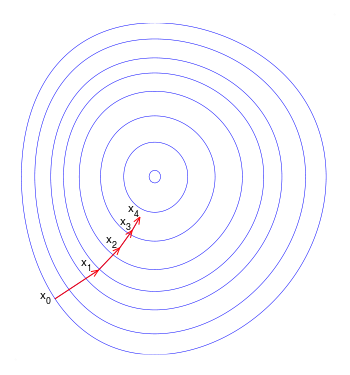
\includegraphics[width=0.9\linewidth]{gradient_descent.png} 
\caption{Наглядное представление метода}
\label{fig:wrapfig}
\end{wrapfigure}

Другой, не менее изветсный метод многомерной оптимизации - \textbf{градиентный спуск}. На каждой итерации вычисляется градиент функции в текущей точке, вдоль которого происходит поиск минимума вдоль направления.\\

\begin{remark*}
Алгоритм требует вычисления градиента функции в точке, поэтому необходимо, чтобы функция была дифференцируемой.\\
\end{remark*}

\begin{algo*}
Пусть целевая функция имеет вид:
$f(x): \mathbb{X} \rightarrow \mathbb{R}$, где $\mathbb{X} \subset \mathbb{R}^n$

Задача оптимизации задана в следующем виде:
найти $x_{opt}:f(x_{opt}) = \min\limits_{x\in \mathbb{X}}f(x) = \mu$


\begin{itemize}
    \item Задать начальное приближение и точность расчёта: $X_0, \varepsilon$
    \item Рассчитать $x^{j+1}=x^{j}-\lambda^{j} \nabla F\left(x^{j}\right)$
    \item Проверить условие остановки (на усмотрение):
    \begin{itemize}
        \item $|x^{j}-x^{j+1}|<\varepsilon$
        \item $|F(x^{j})-F(x^{j+1})|
        <\varepsilon$
        \item $\|\nabla F(x^{i})\|<\varepsilon$
        \item иначе перейти к пункту 2
    \end{itemize}
\end{itemize}

\end{algo*}

\begin{remark*}
$x^{j+1}=x^{j}-\lambda^{j} \nabla F\left(x^{j}\right)$, где $\lambda ^{j}$ задает скорость градиентного спуска и может быть выбрана как:
\begin{itemize}
    \item постоянная, тогда метод может не сходиться
    \item убывать по какому-то закону
    \item гарантировать наискорейший спуск\\
\end{itemize}
\end{remark*}


\textbf{Модификация: метод наискорейшего спуска}

В случае наискорейшего спуска $\lambda^{j}$ определяется как:
$$\lambda^{j}=\underset{\lambda}{\mathrm{argmin}} F\left(x^{j+1}\right) = \underset{\lambda}{\mathrm{argmin}}F\left(x^{j}-\lambda \nabla F\left(x^{j}\right)\right)$$

\begin{remark*}
Чтобы вычислить $\lambda^{j}$, будем использовать метод золотого сечения и алгоритм Moore-Skelboe.
\end{remark*}